\section{Zernike modes: orthogonal coordinates on a pupil disk}
\subsection{Introduction to the map atlas}
A Zernike map plots a \emph{basis function on the pupil}, not image brightness. In Fig.~\ref{fig:atlas}, each disk has normalized radius one; horizontal and vertical axes are $u$ and $v$. Colours encode the signed dimensionless value of $Z_n^m$, with the \emph{same colour scale in every panel}. Multiplying a map by coefficient $c_n^m$ gives that mode's wavefront error in length units. The associated phase is $2\pi c_n^mZ_n^m/\lambda_0$.

The two indices have different roles: $n$ is radial polynomial degree, and $|m|$ counts the angular frequency. Positive $m$ denotes a cosine, negative $m$ a sine, and $m=0$ a circularly symmetric map in our convention. Changing the sign of a coefficient reverses the colours. Rotating a mode mixes its sine and cosine partners. Red and blue are opposite OPD signs, not bright and dark parts of a point image.

All displayed modes have $\avg{Z^2}=1$. Nonpiston modes also have zero mean, so $W=cZ$ has piston-removed RMS $|c|$. Piston itself has mean-square one but zero piston-removed RMS. Unit RMS does not mean unit peak or equal peak-to-valley range.

\begin{figure}[H]\centering
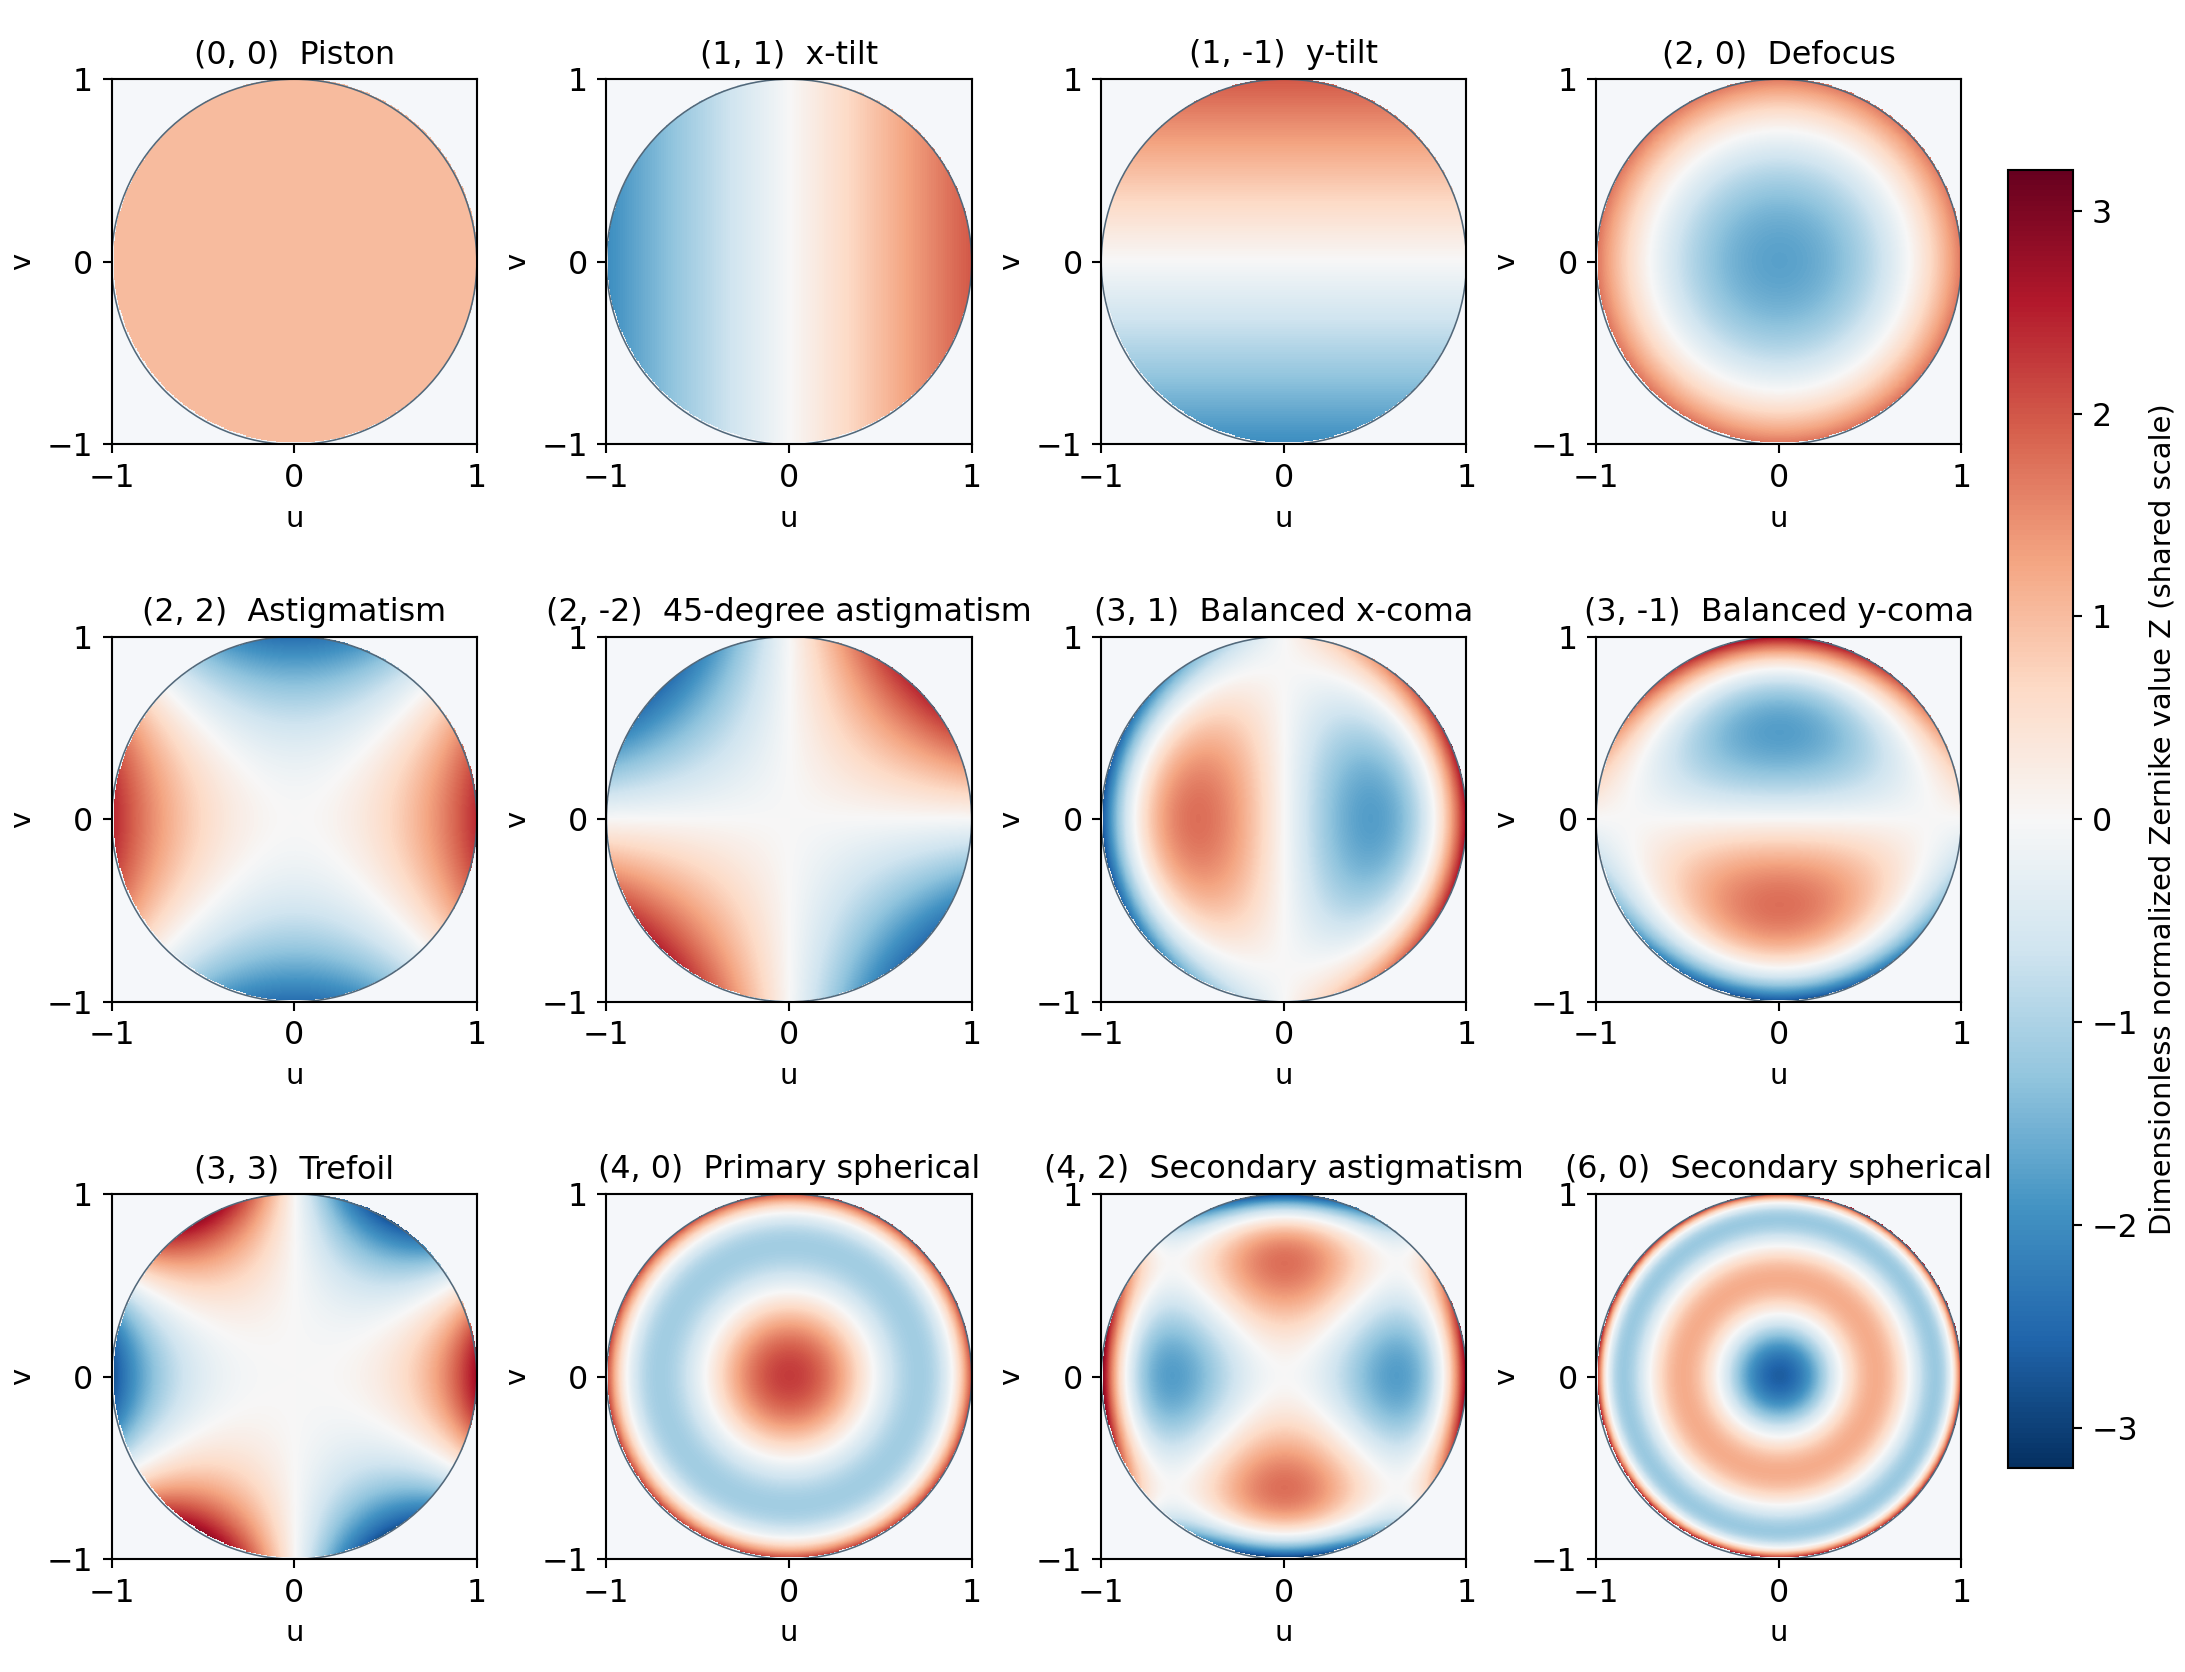
\includegraphics[width=.98\textwidth]{figures/zernike_atlas.png}
\caption{Zernike pupil-map atlas: the 12 selected modes in the supplied explanation, in the same three-row, four-column order. The labels are $(n,m)$, not a single-index numbering scheme. The numerical colour bar runs from $-3.2$ to $+3.2$ in dimensionless normalized $Z_n^m$ values, with zero at white. These are analytic polynomials sampled on a disk; the surrounding area lies outside the pupil.}
\label{fig:atlas}
\end{figure}


\newpage
\subsection{Identification of all 12 panels: read each row left to right}
\begin{longtable}{@{}p{.10\textwidth}p{.10\textwidth}p{.29\textwidth}p{.43\textwidth}@{}}
\toprule Position & $(n,m)$ & Mode & What you see\\\midrule\endhead
R1, C1 & $(0,0)$ & Piston & One constant colour everywhere.\\
R1, C2 & $(1,1)$ & Horizontal or $x$-tilt & Blue on the left, red on the right.\\
R1, C3 & $(1,-1)$ & Vertical or $y$-tilt & Red at the top, blue at the bottom.\\
R1, C4 & $(2,0)$ & Defocus & Blue centre and red outer region.\\
R2, C1 & $(2,2)$ & Primary astigmatism, aligned with coordinate axes & Red left/right and blue top/bottom.\\
R2, C2 & $(2,-2)$ & Primary astigmatism, rotated $45^\circ$ & Alternating signs in diagonal quadrants.\\
R2, C3 & $(3,1)$ & Balanced $x$-coma & Left/right structure with a radial sign reversal.\\
R2, C4 & $(3,-1)$ & Balanced $y$-coma & The corresponding top/bottom structure.\\
R3, C1 & $(3,3)$ & Trefoil & Three red and three blue angular sectors.\\
R3, C2 & $(4,0)$ & Balanced primary spherical aberration & Red centre, blue annulus, red rim.\\
R3, C3 & $(4,2)$ & Secondary astigmatism & Astigmatic angular structure with an additional radial reversal.\\
R3, C4 & $(6,0)$ & Balanced secondary spherical aberration & Alternating concentric regions, beginning blue at the centre.\\\bottomrule
\end{longtable}
This identification follows the supplied atlas explanation. Higher radial degrees introduce additional radial structure within an angular family. The twelve selected modes are an atlas, not a complete sequence through degree six.

\textbf{Why the appearances follow from the formulas.} Tilt is proportional to $u$ or $v$. Defocus changes sign where $2\rho^2-1=0$, at $\rho=1/\sqrt2$. Astigmatism's $\cos2\theta$ or $\sin2\theta$ alternates sign four times around the rim. Coma has radial factor $\rho(3\rho^2-2)$, which reverses sign at $\rho=\sqrt{2/3}$, while its $m=1$ factor makes left/right or top/bottom lobes. Trefoil's $\cos3\theta$ produces six alternating sectors.

Primary spherical's $6\rho^4-6\rho^2+1$ has zeros at
$\rho^2=(3\pm\sqrt3)/6$ and is positive both at the centre and rim. Secondary astigmatism has $\rho^2(4\rho^2-3)$, so its extra radial reversal is at $\rho=\sqrt3/2$. Finally,
\begin{equation}
Z_6^0=\sqrt7(20\rho^6-30\rho^4+12\rho^2-1)
=\sqrt7P_3(2\rho^2-1).
\end{equation}
Its three radial zeros satisfy $\rho^2=(1-\sqrt{3/5})/2,\ 1/2,\ (1+\sqrt{3/5})/2$. The centre value is negative and the rim value positive, explaining the alternating concentric colours.

\subsection{Why raw monomials are inconvenient}
On a uniform unit disk,
\begin{equation}
(f,g)=\avg{fg}=\frac1\pi\int_0^{2\pi}\int_0^1fg\rho\dd\rho\dd\theta,
\qquad \avg{\rho^{2q}}=2\int_0^1\rho^{2q+1}\dd\rho=\frac1{q+1}.
\end{equation}
Thus $(1,\rho^2)=1/2$ and $(\rho^2,\rho^4)=1/4$: the simple powers are not orthogonal. An orthonormal basis makes the coefficients independent under this pupil-area inner product. It does not make their \emph{image effects} independent.

\subsection{Constructing familiar modes by subtracting overlaps}
\textbf{Piston and tilt.} $Z_0^0=1$. Because $\avg{u^2}=\avg{v^2}=1/4$, the normalized tilts are $Z_1^1=2u$ and $Z_1^{-1}=2v$.

\textbf{Defocus.} Subtract the mean of $\rho^2$: $\rho^2-1/2$. Its mean square is $1/3-1/4=1/12$, giving
\begin{equation}
Z_2^0=\sqrt3(2\rho^2-1).
\end{equation}
\textbf{Astigmatism.} Angular averaging makes $\rho^2\cos2\theta$ orthogonal to piston and defocus, and
$\avg{\rho^4\cos^22\theta}=\tfrac12\cdot\tfrac13=1/6$. Therefore
\begin{equation}
Z_2^2=\sqrt6\rho^2\cos2\theta=\sqrt6(u^2-v^2),\qquad
Z_2^{-2}=\sqrt6\rho^2\sin2\theta=2\sqrt6uv.
\end{equation}
\textbf{Coma.} Start from $(\rho^3-b\rho)\cos\theta$ and remove its tilt overlap:
\begin{equation}
0=\avg{(\rho^3-b\rho)\rho\cos^2\theta}
=\frac12\left(\frac13-\frac b2\right),\qquad b=\frac23.
\end{equation}
Multiplying the radial factor by three makes its rim value one. Its real-mode norm is $1/8$, so
\begin{equation}
Z_3^1=\sqrt8(3\rho^3-2\rho)\cos\theta
=\sqrt8(3u\rho^2-2u).
\end{equation}
\textbf{Spherical aberration.} Orthogonalize $\rho^4+b\rho^2+c$ to $1$ and $\rho^2$:
\begin{equation}
\frac13+\frac b2+c=0,\qquad
\frac14+\frac b3+\frac c2=0
\quad\Longrightarrow\quad b=-1,\ c=\frac16.
\end{equation}
Rim normalization and unit mean square give
\begin{equation}
Z_4^0=\sqrt5(6\rho^4-6\rho^2+1).
\end{equation}
The lower-order terms in balanced coma and spherical aberration enforce orthogonality; they are not accidental corrections to an otherwise pure monomial.

\subsection{Deriving the selection rules from integer-order polynomials}
The starting requirement is a real, single-valued wavefront expanded in ordinary Cartesian polynomials $u^pv^q$, with nonnegative integer powers. Angular periodicity alone requires integer Fourier order: $\ee^{\ii m(\theta+2\pi)}=\ee^{\ii m\theta}$ implies $m\in\mathbb Z$. Polynomial regularity at the pupil centre imposes the additional radial restrictions.

Define $z=u+\ii v=\rho\ee^{\ii\theta}$ and $\bar z=u-\ii v=\rho\ee^{-\ii\theta}$. Since $u=(z+\bar z)/2$ and $v=(z-\bar z)/(2\ii)$, these variables span the same polynomial space. A homogeneous term of total degree $n$ can be written as a linear combination of
\begin{equation}
z^p\bar z^q=\rho^{p+q}\ee^{\ii(p-q)\theta},\qquad
p,q\in\{0,1,2,\ldots\},\quad p+q=n.
\end{equation}
Its angular order is $m=p-q$. Solving for the two powers gives
\begin{equation}
p=\frac{n+m}{2},\qquad q=\frac{n-m}{2}.
\end{equation}
Both must be nonnegative integers. Hence
\begin{equation}
\boxed{|m|\leq n,\qquad n-m\ \hbox{even},\qquad
m=-n,-n+2,\ldots,n.}
\end{equation}
Because $m$ and $|m|$ have the same parity, the usual equivalent rule is $n-|m|$ even. Real and imaginary parts give $\cos(|m|\theta)$ and $\sin(|m|\theta)$; for $m=0$, the sine is identically zero, leaving only one mode. This yields $n+1$ real modes at degree $n$.

Conversely, for $M=|m|$ and $n=M+2k$, $k\geq0$,
\begin{equation}
\rho^n\ee^{\ii M\theta}
=(u+\ii v)^M(u^2+v^2)^k,
\end{equation}
which is explicitly a Cartesian polynomial. A lower radial power with the same angular order must still have degree $M+2j$, with $j$ a nonnegative integer. Therefore the full degree-$n$ radial factor at that angular order has the form
\begin{equation}
R_n^M(\rho)=\rho^M\left(a_0+a_1\rho^2+\cdots+a_k\rho^{2k}\right).
\label{eq:selectionform}
\end{equation}
Orthogonalization chooses the $a_j$; it does not invent the allowed powers. In descending order these are $\rho^n,\rho^{n-2},\ldots,\rho^M$, exactly those in the Zernike factorial formula.

For example, degree three allows $m=\pm1,\pm3$: $\rho^3\cos\theta=u(u^2+v^2)$ and $\rho^3\cos3\theta=u^3-3uv^2$ are polynomials. Degree two allows $m=0,\pm2$. The apparently integer-powered expression $\rho^2\cos\theta=u\sqrt{u^2+v^2}$ is not a Cartesian polynomial. Thus an integer radial power alone is insufficient: the angular and radial orders must satisfy the parity and bound together. Nonpolynomial angular functions can still be expanded in the complete Zernike basis; the selection rules define the polynomial basis, not a ban on other physical wavefronts.

\subsection{General definition and the Legendre connection}
Allowed indices satisfy $n\geq0$, $|m|\leq n$, and $n-|m|$ even. Put $M=|m|$ and $k=(n-M)/2$. The radial polynomial is
\begin{equation}
\boxed{R_n^M(\rho)=\sum_{j=0}^{k}
\frac{(-1)^j(n-j)!}{j!(k-j)!(M+k-j)!}\rho^{n-2j}.}
\label{eq:radial}
\end{equation}
Define the normalized real functions by
\begin{equation}
\boxed{Z_n^m=\begin{cases}
\sqrt{n+1}\,R_n^0,&m=0,\\
\sqrt{2(n+1)}\,R_n^m\cos(m\theta),&m>0,\\
\sqrt{2(n+1)}\,R_n^{|m|}\sin(|m|\theta),&m<0.
\end{cases}}
\label{eq:zdef}
\end{equation}
The parity restriction is natural for a polynomial on the disk: a factor $\rho^M\cos M\theta$ or $\rho^M\sin M\theta$ is a homogeneous Cartesian polynomial, and multiplication by powers of $\rho^2=u^2+v^2$ raises its degree by two.

Use $t=\rho^2$ and the shifted weighted Rodrigues construction
\begin{equation}
Q_k^{(M)}(t)=\frac{t^{-M}}{k!}\frac{\dd^k}{\dd t^k}
\left[t^{M+k}(t-1)^k\right],\qquad
R_{M+2k}^M(\rho)=\rho^M Q_k^{(M)}(\rho^2).
\label{eq:rodrigues}
\end{equation}
The derivative contains $t^M$, so $Q_k^{(M)}$ is a degree-$k$ polynomial, not a singular function. At $t=1$, only the term with all $k$ derivatives on $(t-1)^k$ survives, so $R_n^M(1)=1$.

For $M=0$, recall Legendre's Rodrigues formula
\begin{equation}
P_k(x)=\frac{1}{2^k k!}\frac{\dd^k}{\dd x^k}(x^2-1)^k.
\end{equation}
Set $x=2t-1$. Since $(x^2-1)^k=4^kt^k(t-1)^k$ and $\dd/\dd x=\tfrac12\dd/\dd t$, the powers of two cancel:
\begin{equation}
\boxed{R_{2k}^{0}(\rho)=P_k(2\rho^2-1).}
\end{equation}
For example $P_1(x)=x$ gives $2\rho^2-1$, while
$P_2(x)=(3x^2-1)/2$ gives $6\rho^4-6\rho^2+1$.
For general $M$, the correct extension is a Jacobi polynomial:
\begin{equation}
\boxed{R_{M+2k}^{M}(\rho)=\rho^M P_k^{(0,M)}(2\rho^2-1).}
\label{eq:jacobi}
\end{equation}
The $(0,M)$ order refers to Jacobi weight $(1-x)^0(1+x)^M$. After $x=2t-1$, this is proportional to $t^M$, exactly the weight below. Thus only the azimuthally symmetric radial family is directly a shifted Legendre family; replacing all radial factors by ordinary Legendre polynomials would be incorrect. See the linked NIST definitions and Rodrigues formulas in the source record.

\subsection{Derive the factorial formula}
Expand the Rodrigues bracket:
\begin{equation}
t^{M+k}(t-1)^k=\sum_{s=0}^k(-1)^{k-s}\binom{k}{s}t^{M+k+s}.
\end{equation}
Taking $k$ derivatives, multiplying by $t^{-M}/k!$, and then by $\rho^M$ yields
\begin{equation}
R_{M+2k}^M(\rho)=\sum_{s=0}^k
\frac{(-1)^{k-s}(M+k+s)!}{s!(k-s)!(M+s)!}\rho^{M+2s}.
\end{equation}
Set $j=k-s$ and $n=M+2k$ to obtain \eqref{eq:radial}. The factorial expression therefore follows from an orthogonal-polynomial construction rather than being a formula to memorize without context.

\section{Proof of general Zernike orthogonality}
\subsection{Angular orthogonality separates different azimuthal orders}
The identity $\int_0^{2\pi}\ee^{\ii q\theta}\dd\theta=2\pi\delta_{q0}$ follows by integrating the exponential for nonzero integer $q$. Resolving sines and cosines into exponentials gives, for positive integers $M,L$,
\begin{align}
\int_0^{2\pi}\cos M\theta\cos L\theta\dd\theta&=\pi\delta_{ML},\\
\int_0^{2\pi}\sin M\theta\sin L\theta\dd\theta&=\pi\delta_{ML},\\
\int_0^{2\pi}\sin M\theta\cos L\theta\dd\theta&=0.
\end{align}
A constant integrates to $2\pi$, while every nonconstant sine/cosine has zero integral. Only modes with the same angular type and frequency can have a nonzero inner product. It remains to distinguish their radial degrees.

\subsection{Radial orthogonality at fixed angular order}
Let $F_k(t)=t^{M+k}(t-1)^k$ and take $\ell<k$. Because $\rho\dd\rho=\dd t/2$,
\begin{align}
\int_0^1R_{M+2k}^M R_{M+2\ell}^M\rho\dd\rho
&=\frac12\int_0^1t^M Q_k^{(M)}Q_\ell^{(M)}\dd t\\
&=\frac{1}{2k!}\int_0^1Q_\ell^{(M)}F_k^{(k)}\dd t.
\end{align}
Integrate by parts $k$ times. Every endpoint term contains a derivative of $F_k$ of order at most $k-1$. Such derivatives vanish at both ends: $F_k$ has a zero of order $M+k\geq k$ at zero and of order $k$ at one. The integral becomes
\begin{equation}
\frac{(-1)^k}{2k!}\int_0^1
\frac{\dd^k Q_\ell^{(M)}}{\dd t^k}\,F_k(t)\dd t=0,
\end{equation}
because $Q_\ell^{(M)}$ has degree $\ell<k$. Symmetry of the inner product handles $k<\ell$. This proves orthogonality for all unequal radial degrees at fixed $M$, including the endpoints rather than merely asserting their cancellation.

\subsection{Compute the radial norm, not just the zero overlaps}
The highest coefficient of $Q_k^{(M)}$ is
\begin{equation}
A_k=\frac{(M+2k)!}{k!(M+k)!},\qquad
\frac{\dd^kQ_k^{(M)}}{\dd t^k}=k!A_k.
\end{equation}
Perform the same $k$ integrations by parts with $\ell=k$:
\begin{align}
\int_0^1[R_{M+2k}^M]^2\rho\dd\rho
&=\frac{A_k}{2}\int_0^1t^{M+k}(1-t)^k\dd t\\
&=\frac{A_k}{2}\frac{(M+k)!k!}{(M+2k+1)!}
=\boxed{\frac1{2(n+1)}}.
\end{align}
For completeness, $B(a,b)=\int_0^1t^a(1-t)^b\dd t$ obeys
$B(a,b)=b\,B(a+1,b-1)/(a+1)$ by integration by parts; iterating to
$B(a+b,0)=1/(a+b+1)$ gives $a!b!/(a+b+1)!$ for nonnegative integers.

Combining zero overlaps and the norm,
\begin{equation}
\int_0^1R_n^M R_{n'}^M\rho\dd\rho
=\frac{\delta_{nn'}}{2(n+1)}.
\end{equation}
Multiply by the angular norm and divide by pupil area $\pi$. For $m=0$, the unnormalized norm is $1/(n+1)$; for a nonzero sine/cosine it is $1/[2(n+1)]$. The square-root factors in \eqref{eq:zdef} therefore give
\begin{equation}
\boxed{\avg{Z_n^mZ_{n'}^{m'}}=\delta_{nn'}\delta_{mm'}.}
\label{eq:orth}
\end{equation}
This proves orthogonality and normalization for every allowed real mode. Completeness is a separate statement: these modes span all Cartesian polynomial restrictions on the disk, since their leading radial terms are nonzero and the lower terms form a triangular change of basis. Polynomials are dense in the disk's $L^2$ space, so the full mode family is complete there. A finite truncation retains only its corresponding polynomial subspace.

\section{Typical aberrations in Zernike form}
\begin{center}\small
\begin{tabularx}{\textwidth}{@{}l l Y@{}}\toprule
Name & Mode & Normalized polynomial\\\midrule
Piston & $(0,0)$ & $1$\\
$x,y$ tilt & $(1,\pm1)$ & $2\rho\cos\theta$, $2\rho\sin\theta$\\
Defocus & $(2,0)$ & $\sqrt3(2\rho^2-1)$\\
Astigmatism & $(2,\pm2)$ & $\sqrt6\rho^2\cos2\theta$, $\sqrt6\rho^2\sin2\theta$\\
Balanced coma & $(3,\pm1)$ & $\sqrt8(3\rho^3-2\rho)\{\cos\theta,\sin\theta\}$\\
Trefoil & $(3,\pm3)$ & $\sqrt8\rho^3\{\cos3\theta,\sin3\theta\}$\\
Balanced spherical & $(4,0)$ & $\sqrt5(6\rho^4-6\rho^2+1)$\\
Secondary astigmatism & $(4,\pm2)$ & $\sqrt{10}(4\rho^4-3\rho^2)\{\cos2\theta,\sin2\theta\}$\\
Quadrafoil & $(4,\pm4)$ & $\sqrt{10}\rho^4\{\cos4\theta,\sin4\theta\}$\\\bottomrule
\end{tabularx}\end{center}
Here $\pm m$ means cosine first, sine second. Trefoil and quadrafoil are useful pupil modes but are not additional members of the five centred-system Seidel families in \eqref{eq:seidel}.

\subsection{Convert raw Seidel monomials into balanced modes}
Direct rearrangement of the preceding polynomials gives
\begin{align}
u&=\tfrac12 Z_1^1,&
\rho^2&=\tfrac12 Z_0^0+\tfrac1{2\sqrt3}Z_2^0,\\
u\rho^2&=\tfrac13 Z_1^1+\tfrac1{3\sqrt8}Z_3^1,&
\rho^4&=\tfrac13 Z_0^0+\tfrac1{2\sqrt3}Z_2^0+\tfrac1{6\sqrt5}Z_4^0,\\
u^2&=\tfrac14 Z_0^0+\tfrac1{4\sqrt3}Z_2^0+\tfrac1{2\sqrt6}Z_2^2.
\end{align}
In these lines $u$ is the Cartesian pupil coordinate (not a spatial frequency). Therefore $A\rho^4$ includes piston and defocus as well as balanced spherical; $Bh\,u\rho^2$ includes tilt as well as balanced coma; $Ch^2u^2$ includes defocus and piston as well as balanced astigmatism. Field curvature is a field-dependent defocus coefficient; distortion is a field-dependent tilt coefficient. They do not require special new local Zernike shapes.

\subsection{Use the same slope rule on balanced modes}
For $W=cZ_n^m$ and dimensionless image coordinate $\mathbf s=\NA\mathbf x/\lambda_0$, the ray displacement is $(c/\lambda_0)\nabla Z_n^m$. Explicit examples are
\begin{align}
\nabla Z_1^1&=(2,0),&
\nabla Z_2^0&=4\sqrt3(u,v),\\
\nabla Z_2^2&=2\sqrt6(u,-v),&
\nabla Z_2^{-2}&=2\sqrt6(v,u),\\
\nabla Z_3^1&=\sqrt8(9u^2+3v^2-2,6uv),\\
\nabla Z_4^0&=12\sqrt5(2\rho^2-1)(u,v).
\end{align}
These are the analytic gradients used in the ray panels. They make the subtraction of tilt/defocus visible as a change of ray position or focal setting, rather than a change in the diffraction law.

\subsection{Coefficients, RMS, and what balancing means}
Expand $W=\sum c_n^mZ_n^m$. Multiply by one mode and apply \eqref{eq:orth}:
\begin{equation}
\boxed{c_n^m=\avg{WZ_n^m},\qquad
\avg W=c_0^0,\qquad
\sigma_W^2=\sum_{(n,m)\ne(0,0)}(c_n^m)^2.}
\end{equation}
For a finite projection, add the residual mean square if it has not been represented; it is orthogonal to the retained modes. Other deliberately removed modes must also be excluded from the quoted residual RMS. These relations assume the full uniformly weighted disk and the stated normalization.

For raw spherical error $A\rho^4$, allow a compensating $d\rho^2$ and then remove piston. The variance is
\begin{equation}
V(d)=\frac{4A^2}{45}+\frac{d^2}{12}+\frac{Ad}{6}.
\end{equation}
Since $V'(d)=(d+A)/6$, the minimum occurs at $d=-A$. The balanced residual is
\begin{equation}
W_{\rm bal}=A(\rho^4-\rho^2+1/6)=\frac{A}{6\sqrt5}Z_4^0,
\qquad \sigma_{\rm bal}=\frac{|A|}{\sqrt{180}}.
\end{equation}
This is four times smaller than the piston-removed RMS of raw $A\rho^4$. It is a meaningful improvement only when the compensating focus adjustment is allowed. Minimizing pupil RMS also need not optimize every image metric.

\textbf{Orientation and measurement.} A pair $c_c\cos M\theta+c_s\sin M\theta$ equals
$C\cos[M(\theta-\theta_0)]$, where $C=\sqrt{c_c^2+c_s^2}$ and
$\theta_0=\operatorname{atan2}(c_s,c_c)/M$. The orientation changes under axis rotation; the pair's norm does not. For obscured pupils or nonuniform weights, the Gram matrix is generally not the identity. Sampled fitting solves
$(B^TQB)\mathbf c=B^TQ\mathbf w$, preferably using QR/SVD numerically; simply summing squared exported coefficients is then not automatically the physical RMS.

Finally, a single index such as $Z_{20}$ is not a unique physical name. Noll, Fringe, OSA/ANSI and simulator conventions differ in order, sign, and normalization. Use $(n,m)$ and the explicit polynomial to make these notes reproducible.

